\chapter{Introducción}
\section{INTRODUCCIÓN}
En los últimos años, gracias al gran desarrollo tecnológico que se ha vivido tanto a nivel de computo (mejorando la eficiencia y el uso de los recursos disponibles) como a nivel de transmisión de datos (mejorando las comunicaciones), ha permitido a las organizaciones el almacenamiento de una gran cantidad de información.

Un ejemplo de esta evolución se puede observar en las figuras (\ref{fig:procPerformance} y \ref{fig:bandwidth-growth}), las millones de instrucciones por segundo (MIPS) que realiza un procesador (relacionado con el tiempo de cómputo) y la velocidad de transmisión de datos en bits por segundo (BPS) han crecido a lo largo de los últimos años \cite{Nielsen2018}. 

\begin{figure*}[htb]
	\centering
	\caption{Velocidad Procesador (MIPS) a lo largo del tiempo. (Fuente: Kurzweil http://www.kurzweilai.net)}
	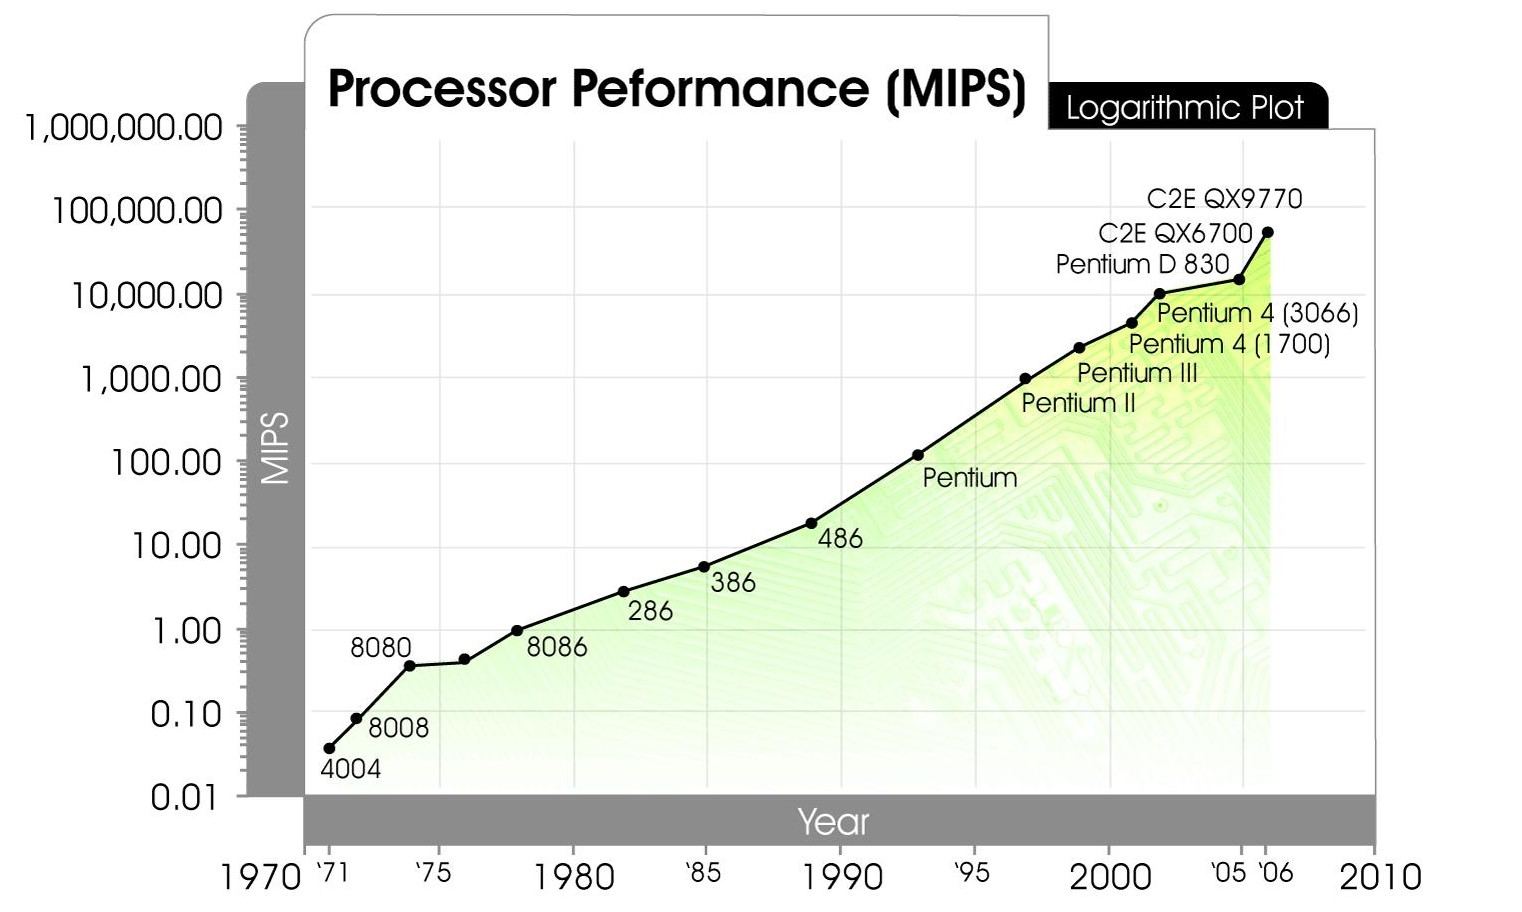
\includegraphics[width=0.6\textwidth]{recursos/processor_performance}
	\label{fig:procPerformance}
\end{figure*}
\FloatBarrier
\begin{figure*}[htb]
	\centering
\caption{Velocidad de transferencia a lo largo del tiempo. (Fuente: Nielsen Norman Group)}
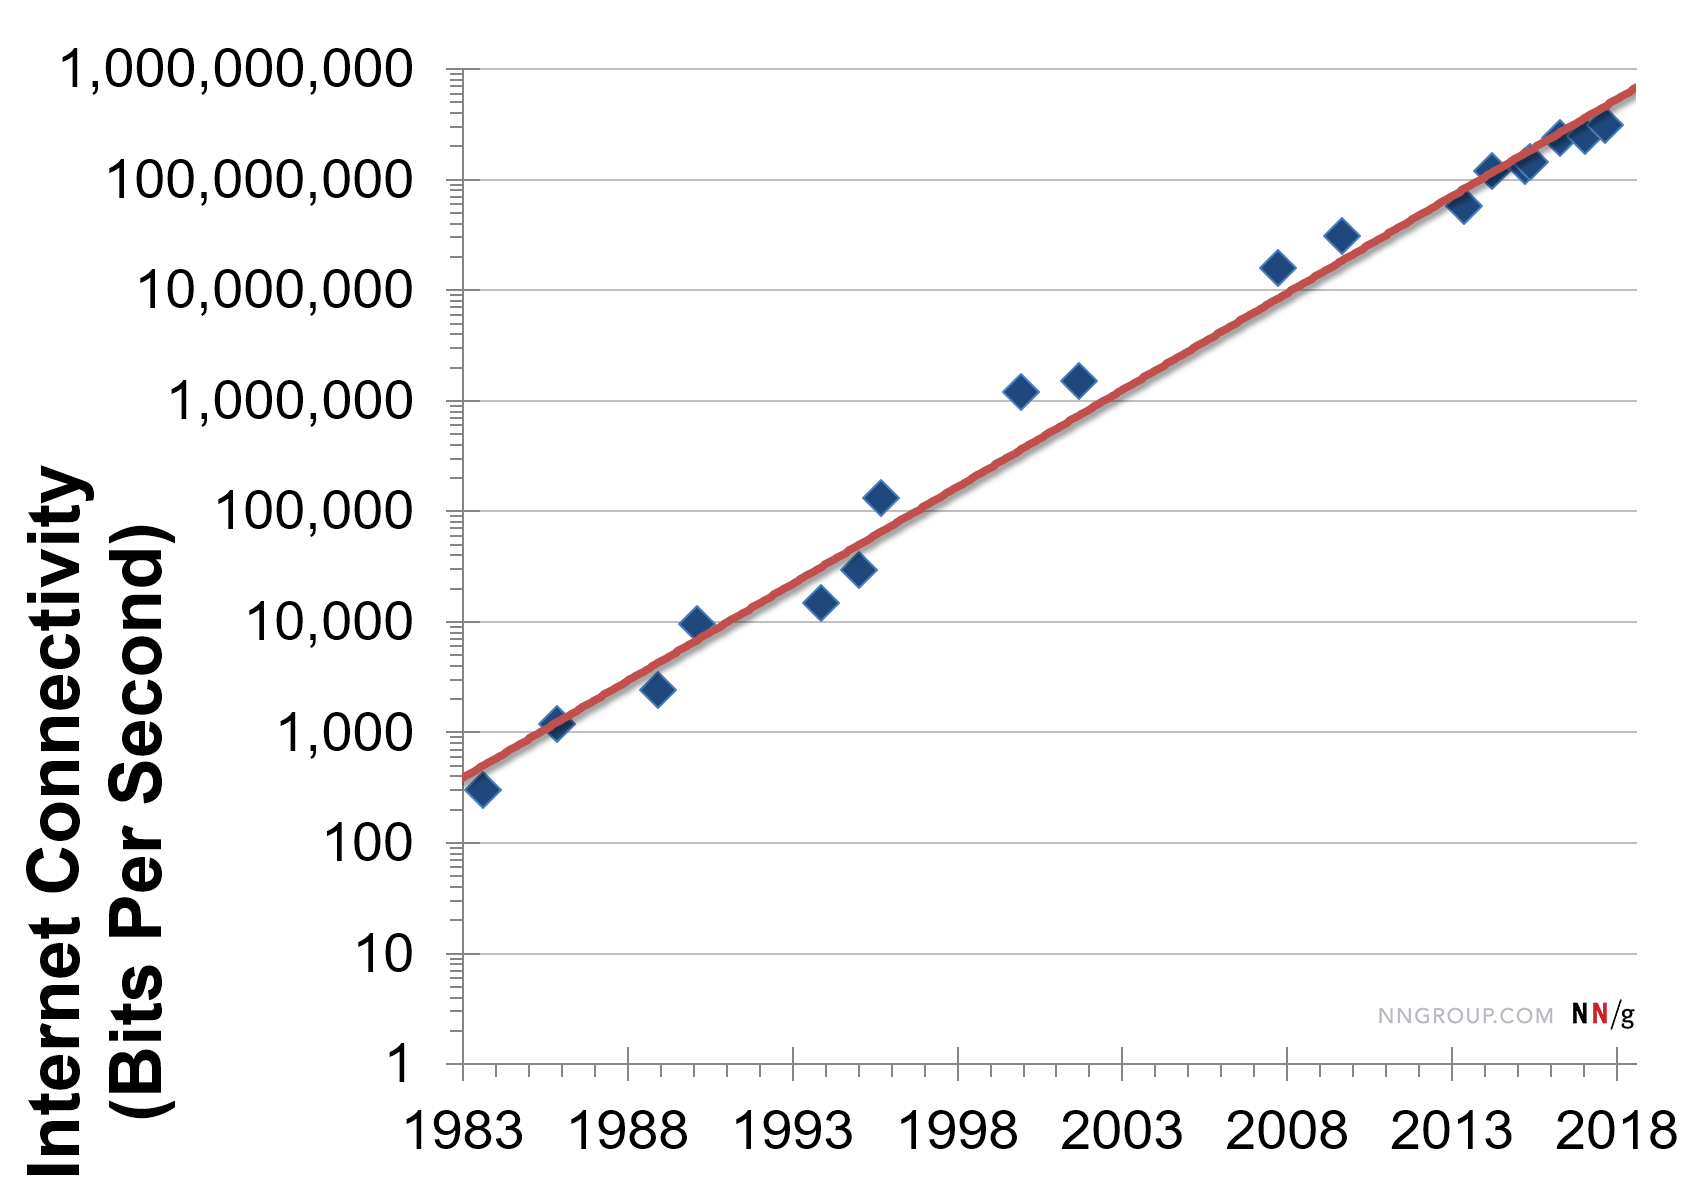
\includegraphics[width=0.5\textwidth]{recursos/bandwidth-growth-nielsen-law}
\label{fig:bandwidth-growth}
\end{figure*}
\FloatBarrier
Para comprender mejor este gran volumen de información que disponen las organizaciones, es necesario utilizar métodos, técnicas, herramientas además de personas con conocimientos (formando todas esta un vínculo estrecho) que permita y ayude a explotar, investigar, predecir y obtener información relevante para tomar decisiones de forma adecuada.

Para descubrir la información en estos grandes volúmenes de datos, es necesario abordar el concepto de minería de datos.  Según \citeA{martinez2016mineria}, la minería de datos es el ``proceso que permite transformar información en conocimiento útil para el
negocio, a través del descubrimiento y cuantificación de relaciones en una
gran base de datos". La minería de datos aplica técnicas estadísticas y matemáticas para poder obtener esta información implícita en los datos.

Algunas de las aplicaciones de la minería de datos según \cite{riquelme2006mineria} son:  comercio y banca, medicina y farmacia, seguridad y detección de fraude, astronomía, geología, minería, agricultura, pesca, ciencias ambientales y ciencias sociales.


\section{Contexto}
Las organizaciones de ámbito educativo no han quedado ajenas a estas necesidades de una mejor comprensión de los datos. Según \citeA{romero2010educational} la minería de datos educativa (EDM) se encarga del desarrollo de métodos para explotar los datos del entorno educativo y entender mejor a los estudiantes y las herramientas que se utilizan para el aprendizaje de estos.

Por un lado, tanto el software educativo como las bases de datos institucionales, han generado una gran cantidad de datos acerca de alumnos, reflejando el aprendizaje de estos a lo largo del tiempo. Por otro, el uso pedagógico de Internet (eLearning), ha generado también grandes cantidades de datos acerca de la enseñanza-aprendizaje (técnicas, herramientas, etc). "Toda esta información es una mina de oro, en el contexto educativo". \cite{romero2010educational}.

\citeA{MOHAMAD2013320} define EDM como una disciplina emergente, relacionada con el desarrollo de métodos para la exploración  de datos que proceden del entorno educativo, para entender mejor a los estudiantes y las herramientas que estos utilizan para aprender. Coincide con el articulo de \citeA{inbook} en el que se indica que la EDM se ha desarrollado mas lentamente que en el resto de ámbitos.
%\citeA{romero2010educational} afirma que el proceso de EDM convierte los datos en bruto, obtenidos de sistemas educativos, en información útil que puede tener un gran impacto en las investigaciones y practicas educativas. No obstante, como se indica en el libro de \cite{inbook} la EDM se ha desarrollado mas lentamente que en el resto de ámbitos.

Como se puede observar en el articulo de \citeA{sin2015application} y en la figura \ref{fig:artPublicados}, el numero de artículos publicados en la conferencia internacional sobre la minería de datos ha crecido desde 2011 casi exponencialmente.

Este aumento de artículos publicados muestra como existe un aumento en el uso de la minería de datos en la educación.

\begin{figure*}[htb]
	\centering
	\caption{Artículos aceptados y publicados desde 2011. Recuperado de \protect\citeA{sin2015application}}
	\includegraphics[width=0.6\textwidth]{recursos/artPublicados}
	\label{fig:artPublicados}
\end{figure*}
\FloatBarrier

A su vez, \citeA{sin2015application}, ha categorizado los artículos publicados según su contenido en categorías que definen las distintas aplicaciones de la minería de datos en la educación. Algunas de estas categorías son: detección de comportamiento, estimación de habilidades, predicción de mejora académica, etc. Por tanto, como se puede observar, dentro de la minería de datos en el entorno educativo, existen distintos campos estudiados y distintos ámbitos de aplicación.


\begin{comment}
Desde la Consejería de Educación de Madrid se están realizando proyectos para conseguir sacar la máxima información del gran número de datos que se poseen.


Obviamente, debido a este gran tamaño de datos, es necesario utilizar métodos, herramientas y personas con conocimientos para obtener información concreta en un tiempo legible. Desde la Consejería de Educación se quiere tener conocimientos actuales sobre la situación educativa. Un ejemplo podría ser el número de alumnos matriculados con necesidades educativas para un determinado centro de la Dirección de Área Territorial Sur. No solo eso, también podrían obtenerse alumnos de un determinado nivel educativo o incluso grupos.


%http://www.superiorinfotech.com/bidw.html
\begin{figure*}[htb]
	\centering
	\caption{
		Arquitectura de un almacén de datos. Recuperado de: Superior Information Technology.
	}
	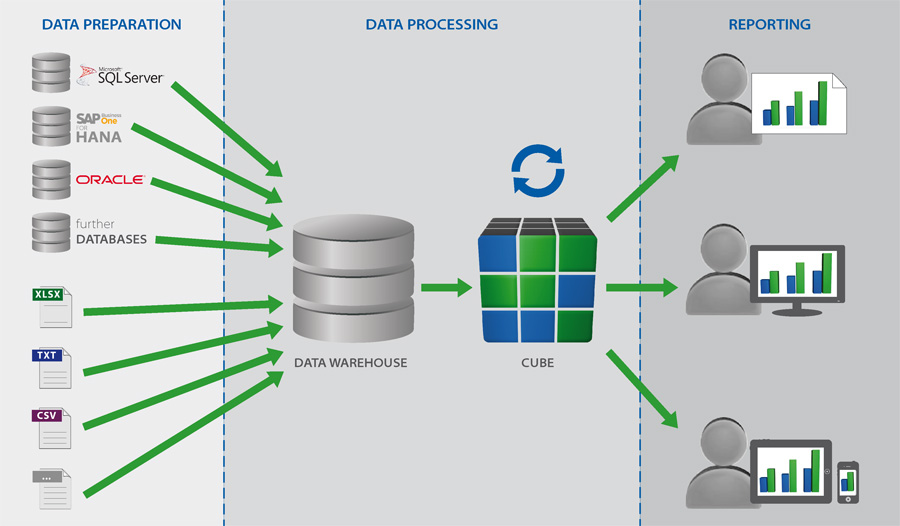
\includegraphics[width=0.6\textwidth]{recursos/arquitecturaDatawarehouse}
	\label{fig:ArqDWH}
\end{figure*}

En la figura \ref{fig:ArqDWH} se pude observar la arquitectura de un almacén de datos. Mediante esta arquitectura, los usuarios finales pueden obtener mucha información sin necesidad de realizar consultas complejas a bases de datos.

No obstante, mostrar la información actual o pasada no es suficiente. La Consejería de Educación también requiere obtener datos futuros. En este aspecto, la Consejería necesita saber cuántos alumnos podrán matricularse en el futuro, con el objetivo de destinar recursos a los centros.
Por tanto, será necesario utilizar técnicas predictivas. Estas técnicas se pueden usar perfectamente en la Consejería puesto que requieren una gran cantidad de datos para realizar pronósticos ajustados, en este sentido, la Consejería tiene un gran histórico de años anteriores.
\end{comment}

\section{Objetivos}
En este trabajo fin de máster se plantea una solución a la necesidad que tiene la Consejería de Educación e Investigación de la Comunidad de Madrid (CEI) para dar respuesta a las necesidades de la demanda concreta de plazas escolares del nuevo período escolar. Para ello, se plantea el uso de herramientas y métodos flexibles que automaticen dichas tareas y proponga, además, nuevas variables o factores que puedan influir en la toma de decisiones. 

Dicho objetivo global se pretende alcanzar mediante los siguientes sub-objetivos:
\begin{itemize}
	\item Seleccionar variables de interés, relativas a la resolución de las necesidades anteriormente expuesta, para estudiar y que aporten valor en el desarrollo de este TFM.
	\item Obtener modelos que se ajusten correctamente a los datos.
	\item Probar distintos modelos y seleccionar aquellos que aporten mayor precisión en la predicción. 
	\item Utilizar los modelos seleccionados para realizar predicciones con los datos existentes. 
\end{itemize}

\section{Metodología}
El proceso o metodologia llevado a cabo en este TFM sigue las siguientes fases:
\begin{enumerate}
	\item En primer lugar, se ha detectado una determinada necesidad en una unidad de la Consejería de Educación e Investigación de la Comunidad de Madrid. \footnote{El autor de este TFM ha colaborado con la Consejería de Educación e Investigación de la Comunidad de Madrid en el desarrollo del proyecto inicial} 
	\item Una vez detectada la necesidad, se realizan reuniones con dicha unidad para obtener la mayor información posible acerca de sus necesidades y la forma en la que satisfacerlas. Antes de comenzar la investigación, se debe tener un claro conocimiento sobre las necesidades existentes y establecer un plan de acción.
	\item A partir del conocimiento sobre cuales son las necesidades, se realiza una propuesta para poder satisfacer dichas necesidades
	\item La propuesta establecida debe ser validada por la propia unidad.
	\item Una vez validada la propuesta, se estudian distintos modelos. Se debe analizar cual de estos es el que mayor precisión obtiene.
	\item Por ultimo, se valida el modelo seleccionado y realizar las predicciones correspondientes con los datos de la unidad.
\end{enumerate}

\section{Organización del TFM}
La estructura que se va a seguir en el TFM es la siguiente:
\begin{itemize}
	\item \textbf{Capítulo 1. Introducción:} En el primer capítulo se definen las necesidades existentes que justifican el desarrollo de este trabajo. También se definen los objetivos que se persiguen con la realización de este. Por último, se presenta la estructura que tiene el presente documento.
	\item \textbf{Capítulo 2. Justificación teórica:} En este segundo capítulo se realiza una investigación sobre el estado de la cuestión, estudiando los métodos, modelos y usos de la minería de datos en el ámbito educativo. 
	\item \textbf{Capítulo 3. Propuesta de intervención:} En este tercer capítulo se define el problema existente.
	\item \textbf{Capítulo 4. Diseño de la investigación:} Este capítulo define los pasos que se siguen en la realización de un proyecto de minería de datos. Se detallan también las tareas que se van a desempeñar en cada uno de los pasos.
	\item \textbf{Capítulo 5. Analisis de los resultados:} Una vez realizado el analisis exploratorio y predictivo, se mostraran los resultados obtenidos en este capitulo.
	\item \textbf{Capítulo 6. Conclusiones:} En este capítulo se detallan las conclusiones obtenidas a partir de los resultados alcanzados.
\end{itemize}




